
\chapter[Lý thuyết và bài tập:\\ Máy phát điện xoay chiều một pha;\\Lý thuyết:\\ Máy phát điện xoay chiều ba pha]{Lý thuyết và bài tập: Máy phát điện xoay chiều một pha;\\	Lý thuyết: Máy phát điện xoay chiều ba pha}
\section{Lý thuyết}
\subsection{Máy phát điện xoay chiều một pha}
\subsubsection{Cấu tạo}
Máy phát điện xoay chiều một pha gồm hai bộ phận chính:
\begin{itemize}
	\item \textbf{Phần cảm}: vành nam châm tròn gồm $p$ cặp cực, tạo ra từ trường. 
	\item \textbf{Phần ứng}: gồm các cuộn dây giống nhau nối với nhau, cố định trên một vòng tròn.  
\end{itemize}
Một trong hai phần đặt cố định, phần còn lại quay quanh một trục. Phần cố định gọi là stato, phần quay gọi là rôto.
\begin{center}
	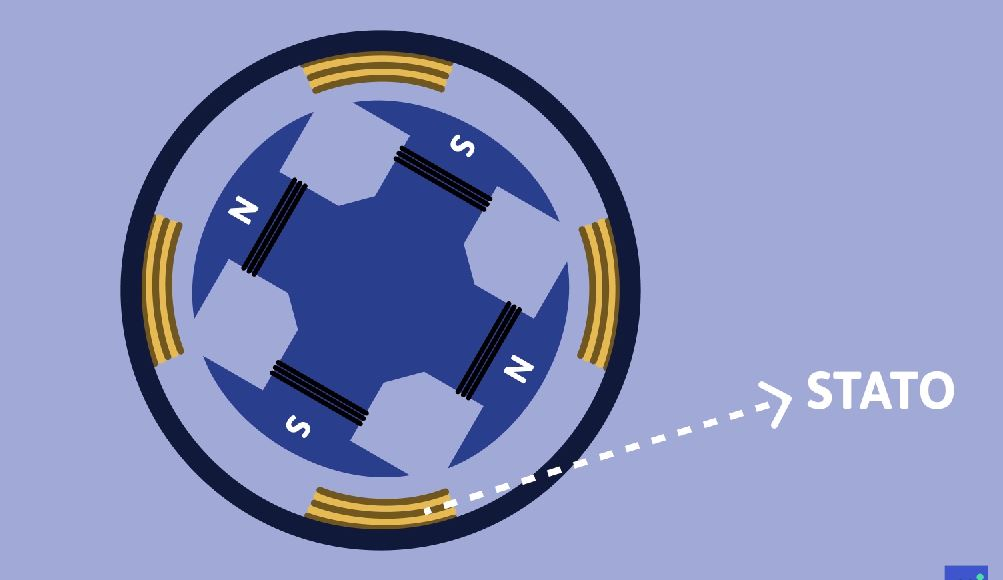
\includegraphics[scale=0.35]{VN12-PH-22-L-015-1-V2-01.jpg}
\end{center}
\subsubsection{Nguyên tắc hoạt động}
Hoạt động dựa trên hiện tượng cảm ứng điện từ.

Khi rôto quay với tốc độ $n$ vòng/giây, từ thông qua các cuộn dây biến thiên tuần hoàn với tần số
\begin{equation*}
	f=np,
\end{equation*}
trong đó:
\begin{itemize}
	\item $f$ là tần số của dòng điện;
	\item $n$ là tốc độ của rôto;
	\item $p$ là số cặp cực.
\end{itemize}
\luuy{Nếu tốc độ quay của rôto là $n$ vòng/phút thì tần số $f$ được tính theo công thức:
	\begin{equation*}
		f=\dfrac{np}{60}.
	\end{equation*}
}

Trên các cuộn dây có suất điện động xoay chiều hình sin với cùng tần số $f$:
\begin{equation*}
	e=\omega NBS\cos(\omega t +\varphi),
\end{equation*}
hoặc:
\begin{equation*}
	e=E_0\cos(\omega t +\varphi),
\end{equation*}
trong đó:
\begin{itemize}
	\item $\omega=2\pi f$ là tần số góc của dòng điện,
	\item $N$ là tổng số vòng dây (của tất cả các cuộn dây),
	\item $B$ là độ lớn cảm ứng từ do phần ứng tạo ra trên cuộn dây,	
	\item $S$ là diện tích mỗi vòng dây,
	\item $E_0$ là suất điện động cực đại.
\end{itemize}



\subsubsection{Dòng một pha}
Mỗi máy phát điện xoay chiều một pha chỉ phát ra một dòng điện, gọi là dòng một pha.
\subsection{Máy phát điện xoay chiều ba pha}
\subsubsection{Cấu tạo}
Máy phát điện xoay chiều ba pha cấu tạo gồm hai phần:			
\begin{itemize}
	\item Stato: ba cuộn dây riêng rẽ giống nhau, quấn trên ba lõi sắt đặt lệch nhau $\dfrac{2\pi}{3}\ \text{rad}$ trên một vòng tròn; 
	\item Rôto: một nam châm điện.
\end{itemize}
\begin{center}
	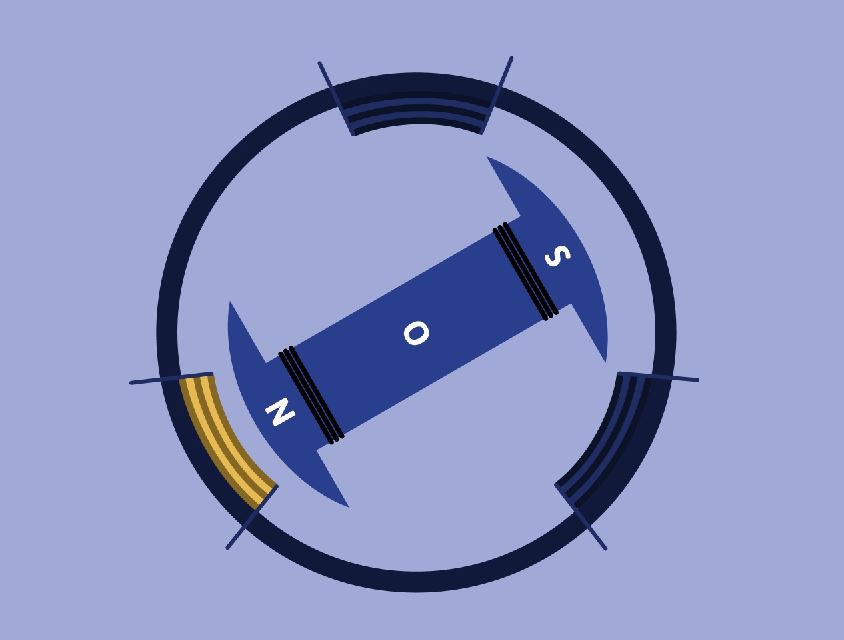
\includegraphics[scale=0.3]{VN12-PH-22-L-015-2-V2-01.jpg}
\end{center}
\subsubsection{Nguyên tắc hoạt động }
Hoạt động dựa trên hiện tượng cảm ứng điện từ.

Khi rôto quay với với tần số $f$ (vòng/giây) thì từ thông qua mỗi cuộn dây đều biến thiên tuần hoàn với tần số $f$, làm xuất hiện trên mỗi cuộn một suất điện động xoay chiều hình sin.

Do ba cuộn dây bị lệch nhau $\dfrac{2\pi}{3}$ rad nên ba suất điện động của ba cuộn dây có cùng tần số, cùng biên độ nhưng lệch pha nhau $\dfrac{2\pi}{3}$
\begin{eqnarray*}
	e_1&=&E_0\cos\omega t,\\
	e_2&=&E_0\cos\left( \omega t -\frac{2\pi}{3}\right) ,\\ e_3&=&E_0\cos\left( \omega t +\frac{2\pi}{3}\right).
\end{eqnarray*}

Máy phát điện xoay chiều ba pha được kí hiệu như sau:
\begin{center}
	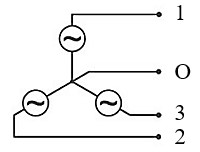
\includegraphics[scale=0.9]{VN12-PH-22-L-015-2-V2-02.jpg}
\end{center}
\subsubsection{Dòng ba pha}
Máy phát điện xoay chiều ba pha phát ra dòng ba pha, là một hệ thống gồm ba dòng điện hình sin cùng tần số, nhưng lệch pha nhau $\dfrac{2\pi}{3}$ từng đôi một. 
\subsubsection{Cách mắc mạch ba pha} 

Mắc hình sao cần 4 dây để nối ba cuộn dây trong máy phát điện xoay chiều ba pha với 3 tải tiêu thụ. 
\begin{center}
	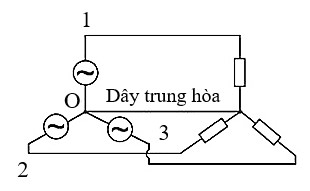
\includegraphics[scale=1.0]{VN12-PH-22-L-015-2-V2-03.jpg}
\end{center}
\begin{equation*}
	I_\text{d}=I_\text{p};\qquad U_\text{d}=\sqrt 3 U_\text{p},
\end{equation*}
trong đó:
\begin{itemize}
	\item $I_\text{d}$ và $I_\text{p}$ lần lượt là cường độ dòng điện dây và cường độ dòng điện pha;
	\item $U_\text{d}$ và $U_\text{p}$ lần lượt là điện áp dây và điện áp điện pha.
\end{itemize}

Mắc tam giác cần 3 dây để nối ba cuộn dây trong máy phát điện xoay chiều ba pha với 3 tải tiêu thụ.
\begin{center}
	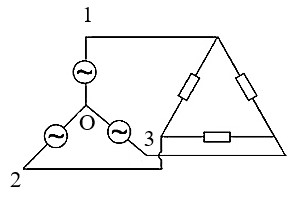
\includegraphics[scale=1.0]{VN12-PH-22-L-015-2-V2-04.jpg}
\end{center}
\begin{equation*}
	I_\text{d}=\sqrt 3 I_\text{p}; \qquad U_\text{d}=U_\text{p}
\end{equation*}
trong đó:
\begin{itemize}
	\item $I_\text{d}$ và $I_\text{p}$ lần lượt là cường độ dòng điện dây và cường độ dòng điện pha;
	\item $U_\text{d}$ và $U_\text{p}$ lần lượt là điện áp dây và điện áp điện pha.
\end{itemize}


\section{Mục tiêu bài học - Ví dụ minh họa}
\begin{dang}{Xác định suất điện động do máy phát điện xoay chiều một pha tạo ra}
	\viduii{2}{Suất điện động do một máy phát điện xoay chiều một pha tạo ra có biểu thức\\ $e=120\sqrt{2}\cos(100\pi t)\,\text{V}$. Giá trị hiệu dụng của suất điện động này bằng
		\begin{mcq} (4)
			\item $\SI{100}{\volt}$.
			\item $\SI{120}{\volt}$.
			\item $120\sqrt{2}\,\text{V}$.
			\item $100\pi\,\text{V}$.
		\end{mcq}
	}
	{	\begin{center}
			\textbf{Hướng dẫn giải}
		\end{center}
		
		Giá trị hiệu dụng của suất điện động này bằng
		\begin{equation*}
			e=\dfrac{E_0}{\sqrt{2}}=\SI{120}{\volt}.
		\end{equation*}
		
		\textbf{Đáp án: B.}
	}
	\viduii{2}{Suất điện động do một máy phát điện xoay chiều một pha tạo ra có biểu thức\\ $e=220\cos(100\pi t+0,25\pi)\,\text{V}$. Giá trị cực đại của suất điện động này là
		\begin{mcq} (4)
			\item $220\sqrt{2}\,\text{V}$.
			\item $110\sqrt{2}\,\text{V}$.
			\item $\SI{110}{\volt}$.
			\item $\SI{220}{\volt}$.
		\end{mcq}
	}
	{	\begin{center}
			\textbf{Hướng dẫn giải}
		\end{center}
		
		Giá trị cực đại của suất điện động này là $\SI{220}{\volt}$.
		
		\textbf{Đáp án: D.}
	}
\end{dang}

\begin{dang}{Xác định tần số, tốc độ quay và số cặp cực của máy phát điện xoay chiều một pha}
	\viduii{1}{Một máy phát điện xoay chiều một pha (kiểu cảm ứng) có $p$ cặp cực, quay đều với tốc độ $n$ vòng/phút, với số cặp cực bằng số cuộn dây của phần ứng thì tần số của dòng điện do máy tạo ra là $f$ Hz. Hệ thức nào sau đây đúng? 
		
		\begin{mcq}(2)
			\item $f=60np$.
			\item $n= \dfrac{60p}{f}$.
			\item $f = \dfrac{60n}{p}$.
			\item $n = \dfrac {60f}{p}$.
		\end{mcq}
	}
	{	\begin{center}
			\textbf{Hướng dẫn giải}
		\end{center}
		
		Tần số của dòng điện do máy phát ra:
		
		$$f = \dfrac{pn}{60} \Rightarrow n =\dfrac{60f}{p}.$$
		
		\textbf{Đáp án: D}.
	}
	\viduii{2}{Một máy phát điện xoay chiều một pha có phần cảm là rôto gồm 4 cặp cực (4 cực Nam và 4 cực Bắc). Để suất điện động do máy này sinh ra có tần số $50\ \text{Hz}$ thì rôto phải quay với tốc độ bao nhiêu?
		\begin{mcq} (2)
			\item $\SI{12.5}{}\,\text{vòng/phút}$.
			\item $25\,\text{vòng/phút}$.
			\item $\SI{37.5}{}\,\text{vòng/phút}$.
			\item $50\,\text{vòng/phút}$.
		\end{mcq}
	}
	{	\begin{center}
			\textbf{Hướng dẫn giải}
		\end{center}
		
		Tốc độ quay của rôto:
		\begin{equation*}
			f=n\cdot p \Rightarrow n=\frac{f}{p}=\SI{12.5}{}\,\text{vòng/phút}.
		\end{equation*}
		\textbf{Đáp án: A.}
	}
	\viduii{3}{Hai máy phát điện xoay chiều một pha đang hoạt động bình thường và tạo ra hai suất điện động có cùng tần số $f$. Rôto của máy thứ nhất có $p_1$ cặp cực và quay với tốc độ $n_1=1800\,\text{vòng/phút}$. Rôto của máy thứ hai có $p_2=4$ cặp cực và quay với tốc độ $n_2$. Biết $n_2$ có giá trị trong khoảng từ $12\,\text{vòng/giây}$ đến $18\,\text{vòng/giây}$. Giá trị của $f$ là
		\begin{mcq} (4)
			\item $\SI{54}{\hertz}$.
			\item $\SI{60}{\hertz}$.
			\item $\SI{48}{\hertz}$.
			\item $\SI{50}{\hertz}$.
		\end{mcq}
	}
	{	\begin{center}
			\textbf{Hướng dẫn giải}
		\end{center}
		
		Hai máy có cùng tần số $f$ nên
		\begin{equation*}
			f=f_1=f_2\Rightarrow p_1n_1=p_2n_2\Rightarrow n_2= n_1\cdot\dfrac{p_1}{p_2}.
		\end{equation*}
		
		Vì $n_2$ có giá trị trong khoảng từ $12\,\text{vòng/giây}$ đến $18\,\text{vòng/giây}$ nên
		\begin{equation*}
			12\,\text{vòng/giây} \leq n_2 \leq 18\,\text{vòng/giây}
		\end{equation*}
		\begin{equation*}
			\Rightarrow 12\,\text{vòng/giây} \leq n_1\cdot\dfrac{p_1}{p_2} \leq 18\,\text{vòng/giây}
		\end{equation*}
		\begin{equation*}
			\Rightarrow 12\,\text{vòng/giây} \leq 30\,\text{vòng/giây}\cdot\dfrac{p_1}{4} \leq 18\,\text{vòng/giây}
		\end{equation*}
		\begin{equation*}
			1,6 \leq p_1 \leq 2,4.
		\end{equation*}
		
		Vì $p$ nguyên nên chọn $p_1=2$.
		Tần số $f$ của hai máy là
		\begin{equation*}
			f=p_1 n_1= 2\cdot 30\,\text{vòng/giây} = \SI{60}{\hertz}.
		\end{equation*}
		\textbf{Đáp án: B.}
	}
\end{dang}
\begin{dang}{Ghi nhớ công thức tính suất điện động của cuộn dây trong máy phát điện\\ xoay chiều ba pha}
	\viduii{2}{Khi máy phát điện ba pha hoạt động, ở thời điểm suất điện động ở một cuộn dây đạt giá trị cực đại $e_1 = E_0$ thì suất điện động ở hai đầu cuộn dây còn lại là:
		
		\begin{mcq}(2)
			\item $e_2 = \dfrac{\sqrt 3 E_0}{2}; e_3 = - \dfrac{\sqrt 3E_0}{2}$.
			\item $e_2 = e_3 =\dfrac{E_0}{\sqrt 2}$.
			\item $e_2 = \dfrac{E_0}{2}; e_3 = - \dfrac{E_0}{2}$.
			\item $e_2 = e_3 =- \dfrac{E_0}{2}$.
		\end{mcq}
	}
	{	\begin{center}
			\textbf{Hướng dẫn giải}
		\end{center}
		
		Suất điện động ở hai đầu mỗi cuộn dây
		
		$$e_1 = E_0 \cos \omega t;$$
		
		$$e_2 = E_0 \cos \left(\omega t + \dfrac{2\pi}{3}\right);$$
		
		$$e_3 = E_0 \cos \left(\omega t - \dfrac{2\pi}{3}\right).$$
		
		Khi $e_1 = E_0$; $\omega t = 2k\pi$ , thay vào biểu thức tính $e_2$ và $e_3$ 
		
		$$e_2 = e_3 =-\dfrac{E_0}{2}.$$
		
		\textbf{Đáp án: D}.
	}
	
	\viduii{3}{Một máy phát điện xoay chiều ba pha đang hoạt động ổng định. Suất điện động trong ba cuộn dây của phần ứng có giá trị  $e_1$, $e_2$ và $e_3$. Ở thời điểm mà $e_1=\SI{30}{\volt}$ thì $\left|e_2-e_3\right|=\SI{30}{\volt}$. Giá trị cực đại của $e_1$ là
		\begin{mcq} (4)
			\item $\SI{40,2}{\volt}$.
			\item $\SI{51,9}{\volt}$.
			\item $\SI{34,6}{\volt}$.
			\item $\SI{45,1}{\volt}$.
		\end{mcq}
	}
	{	\begin{center}
			\textbf{Hướng dẫn giải}
		\end{center}
		
		Giả sử suất điện động trong khung dây có dạng
		\begin{equation*}
			\left\{\begin{array}{ll}{{{e}_{1}}={{E}_{0}}\cos \omega t}&\\{{{e}_{2}}={{E}_{0}}\cos \left( \omega t+\dfrac{2\pi}{3}\right)}&\\{{{e}_{2}}={{E}_{0}}\cos \left( \omega t-\dfrac{2\pi }{3} \right)}&\end{array}\right.
		\end{equation*}
		
		Theo đề bài
		\begin{equation*}
			\left| {{e}_{2}}-{{e}_{3}} \right|=\SI{30}{\volt}
			\Rightarrow {{e}_{2}}-{{e}_{3}}=\pm \SI{30}{\volt}
			\Rightarrow 2{{E}_{0}}\sin \omega t\sin \frac{2\pi }{3}=\pm \SI{30}{\volt}.
		\end{equation*}
		
		Ngoài ra, cũng theo đề bài
		\begin{equation*}
			{{e}_{1}}={{E}_{0}}\cos \omega t =\SI{30}{\volt}.
		\end{equation*}
		
		Ta có hệ phương trình sau
		\begin{equation*}
			\left\{\begin{array}{ll}{-2{{E}_{0}}\sin \omega t\sin \dfrac{2\pi}{3}=\pm \SI{30}{\volt}}&\\{{{E}_{0}}\cos \omega t=\SI{30}{\volt}}&\end{array}\right.
			\Rightarrow \left\{\begin{array}{ll}{{{E}_{0}}\sin \omega t=\pm 10\sqrt{3}\,\text{V}}&\\{{{E}_{0}}\cos \omega t=\SI{30}{\volt}}&\end{array}\right.
			\Rightarrow {{E}_{0}}=20\sqrt{3}\approx \SI{34,6}{\volt}.
		\end{equation*}
		
		\textbf{Đáp án: C}.
	}
	
\end{dang}
\begin{dang}{Sử dụng công thức của hai cách mắc sao và tam giác trong máy phát điện xoay chiều ba pha để xác định đại lượng cần tìm}
	\viduii{2}{Trong mạch điện xoay chiều ba pha, tải mắc hình sao có dây trung hòa, khi một pha tiêu thụ điện bị hở thì cường độ dòng điện trong hai pha còn lại
		
		\begin{mcq} (2)
			\item đều tăng lên.
			\item đều giảm xuống.
			\item không thay đổi.
			\item đều bằng 0.
		\end{mcq}
	}
	{	\begin{center}
			\textbf{Hướng dẫn giải}
		\end{center}
		
		Vì tải mắc hình sao có dây trung hòa, nên các pha độc lập nhau. Do đó, khi một pha tiêu thụ điện bị hở thì cường độ dòng điện trong hai pha còn lại không bị ảnh hưởng, tức là không thay đổi.
		
		\textbf{Đáp án: C.}
	}
	\viduii{3}{Một máy phát điện ba pha mắc hình sao có điện áp hiệu dụng pha $\SI{127}{V}$ và tần số $\SI{50}{Hz}$. Người ta đưa dòng điện xoay chiều ba pha vào ba tải như nhau mắc hình tam giác, mỗi tải có điện trở thuần $\SI{12}{\Omega}$ và độ tự cảm $\SI{51}{mH}$. Xác định tổng công suất cả ba tải tiêu thụ.
		
		\begin{mcq}(4)
			\item $\SI{991}{W}$.
			\item $\SI{3233}{W}$.
			\item $\SI{4356}{W}$.
			\item $\SI{1452}{W}$.
		\end{mcq}
	}
	{	\begin{center}
			\textbf{Hướng dẫn giải}
		\end{center}
		
		Cảm kháng của cuộn dây:
		
		$$Z_L = L\omega =\SI{16}{\Omega}.$$
		
		Tổng trở của mạch:
		
		$$Z =\sqrt {R^2 +Z^2_L}=\SI{20}{\Omega}.$$
		
		Cường độ dòng điện qua ba cuộn dây:
		
		$$I_1 =I_2 =I_3 = \dfrac{U}{Z} = \dfrac{U_\text{p} \sqrt 3}{Z}.$$
		
		Tổng công suất ba tải:
		
		$$P = 3I_1^2 R =\SI{4356}{W}.$$
		
		\textbf{Đáp án: C}.
	}
	\viduii{3}{Một máy phát điện xoay chiều 3 pha khi hoạt động, người ta dùng vôn kế nhiệt để đo điện áp hai đầu một cuộn dây thì số chỉ của nó là $\SI{127}{V}$. Người ta đưa dòng ba pha do máy phát ra vào 3 bóng đèn giống hệt nhau hoạt động với điện áp hiệu dụng $\SI{220}{V}$ thì các đèn đều sáng bình thường. Chọn phương án đúng. 
		
		\begin{mcq}
			\item Máy mắc hình sao, tải mắc hình sao.
			\item Máy mắc hình sao, tải mắc hình tam giác.
			\item Máy mắc hình tam giác, tải mắc hình sao.
			\item Máy mắc hình tam giác, tải mắc hình tam giác.
		\end{mcq}
	}
	{	\begin{center}
			\textbf{Hướng dẫn giải}
		\end{center}
		
		Nếu $U = U_\text{p}$ thì để tải hoạt động bình thường nguồn mắc sao  - tải mắc sao hoặc nguồn tam giác  - tải mắc tam giác.
		
		Nếu $U = \dfrac{U_\text{p}}{\sqrt 3}$ thì để tải hoạt động bình thường nguồn mắc tam giác  - tải mắc sao.
		
		Nếu $U = \sqrt 3 U_\text{p}$ thì để tải hoạt động bình thường nguồn mắc sao  - tải mắc tam giác. $\Rightarrow$ Phù hợp với đề bài.
				
		\textbf{Đáp án: B}.
	}
\end{dang}


